\documentclass[12pt,a4paper]{report}
\usepackage[margin=1in]{geometry}
\usepackage{graphicx}
\usepackage{listings}
\usepackage{xcolor}
\usepackage{hyperref}
\usepackage{amsmath}
\usepackage{amssymb}
\usepackage{fancyhdr}
\usepackage{lastpage}
\usepackage{array}
\usepackage{booktabs}
\usepackage{float}
\usepackage{caption}
\usepackage{subcaption}
\usepackage[utf8]{inputenc}
\usepackage{dirtree}
\usepackage{tikz}
\usetikzlibrary{shapes,arrows,positioning,calc,fit}

% Code listing style
\definecolor{codegreen}{rgb}{0,0.6,0}
\definecolor{codegray}{rgb}{0.5,0.5,0.5}
\definecolor{codepurple}{rgb}{0.58,0,0.82}
\definecolor{backcolour}{rgb}{0.95,0.95,0.92}

\lstdefinestyle{mystyle}{
    backgroundcolor=\color{backcolour},   
    commentstyle=\color{codegreen},
    keywordstyle=\color{magenta},
    numberstyle=\tiny\color{codegray},
    stringstyle=\color{codepurple},
    basicstyle=\ttfamily\footnotesize,
    breakatwhitespace=false,         
    breaklines=true,                 
    captionpos=b,                    
    keepspaces=true,                 
    numbers=left,                    
    numbersep=5pt,                  
    showspaces=false,                
    showstringspaces=false,
    showtabs=false,                  
    tabsize=2
}

\lstset{style=mystyle}

% Hyperref setup
\hypersetup{
    colorlinks=true,
    linkcolor=black,
    filecolor=magenta,      
    urlcolor=blue,
    pdftitle={VaultGuard Project Report},
    pdfpagemode=FullScreen,
}

% Header and Footer
\pagestyle{fancy}
\fancyhf{}
\rhead{\textbf{VaultGuard Project Report}}
\lhead{Information Security Course}
\cfoot{Page \thepage\ of \pageref{LastPage}}

\title{\textbf{VaultGuard: Secure Password Vault with\\SSL/TLS-Secured Multi-Factor Authentication}\\
\vspace{0.5cm}
\large{A Comprehensive Security Implementation Project}}
\author{Ali Tarek}
\date{\today}

\begin{document}

\begin{titlepage}
\centering
\vspace*{2cm}

\textbf{\LARGE VaultGuard: Secure Password Vault with\\SSL/TLS-Secured Multi-Factor Authentication}\\
\vspace{0.5cm}
{\large A Comprehensive Security Implementation Project}

\vspace{2cm}

\section*{Project Team Members}

\begin{table}[H]
\centering
\begin{tabular}{|c|c|}
\hline
\textbf{Name} & \textbf{Student ID} \\
\hline
Ali Tarek & 21P0123 \\
\hline
Omar Tamer Omar & 21P0032 \\
\hline
Ahmed El-Baramouny & 21P0261 \\
\hline
Ahmed Mohamed & 22P0283 \\
\hline
Fatma Ayman & 2100327 \\
\hline
\end{tabular}
\end{table}

\vspace{2cm}

\textbf{Course:} Computer and Network Security\\
\textbf{Institution:} Ain Shams University\\

\vfill

\end{titlepage}

\newpage

\begin{abstract}
This report presents VaultGuard, a secure password vault application implementing enterprise-grade cryptographic techniques and multi-factor authentication. The project demonstrates the practical application of symmetric encryption (AES-256-GCM), key derivation functions (Argon2id), TOTP-based MFA, SSL/TLS secured communication, and integrity verification mechanisms. The system has been thoroughly tested with 24 comprehensive test cases covering all security components. This report details the problem statement, system design, security analysis, implementation methodology, and comprehensive testing results.
\end{abstract}

\tableofcontents
\newpage

\chapter{Executive Summary}

VaultGuard is a single-user password management application designed with security as the primary concern. It combines client-side encryption with server-side multi-factor authentication to provide robust access control while ensuring that sensitive data remains encrypted on the user's device.

\section{Key Achievements}

\begin{itemize}
    \item Implemented AES-256-GCM encryption for all stored credentials
    \item Deployed Argon2id key derivation function for secure master password handling
    \item Integrated TOTP-based MFA with 60-second validity window
    \item Established SSL/TLS secured communication channels
    \item Implemented SHA-256 integrity verification for tamper detection
    \item Developed comprehensive test suite with 24 passing tests
    \item Created user-friendly GUI interfaces for both desktop and mobile authentication
    \item Restructured project architecture for maintainability and scalability
\end{itemize}

\chapter{Problem Statement and Requirements}

\section{Problem Description}

Traditional password managers often face security challenges when passwords are transmitted over networks or stored without proper encryption. Common vulnerabilities include:

\begin{enumerate}
    \item \textbf{Weak Encryption}: Many applications use outdated or weak encryption algorithms
    \item \textbf{Single Factor Authentication}: Reliance on password alone is insufficient
    \item \textbf{Insecure Key Management}: Master passwords often stored as plaintext hashes
    \item \textbf{Plaintext Transmission}: Network communication without encryption
    \item \textbf{Lack of Integrity Checks}: No detection of data tampering
    \item \textbf{User Experience}: Complex security often leads to poor adoption
\end{enumerate}

\section{Project Requirements}

\subsection{Functional Requirements}

\begin{enumerate}
    \item Users must be able to set up a Master Password and register with MFA server
    \item Authentication requires both Master Password and valid TOTP code
    \item Users can add, view, edit, and delete stored credentials
    \item OTP must be valid for exactly 60 seconds
    \item All network communication must use SSL/TLS
    \item Data must be encrypted locally before storage
\end{enumerate}

\subsection{Non-Functional Requirements}

\begin{enumerate}
    \item All sensitive data encrypted at rest and in transit
    \item Strong key derivation using Argon2id
    \item AEAD (Authenticated Encryption with Associated Data)
    \item Integrity verification using SHA-256
    \item Cross-platform compatibility (Windows/Linux)
    \item Responsive user interface
    \item Comprehensive error handling
    \item Audit logging capability
\end{enumerate}

\chapter{System Design and Architecture}

\section{System Overview}

VaultGuard consists of five interconnected components:

\subsection{Component Architecture}

\begin{table}[H]
\centering
\begin{tabular}{|p{3cm}|p{4cm}|p{5cm}|}
\hline
\textbf{Component} & \textbf{Technology} & \textbf{Responsibility} \\
\hline
VaultGuard Client & Python + CustomTkinter & Password management, local encryption, GUI \\
MFA Server & Flask + Python & User registration, OTP validation (HTTPS) \\
Mobile Authenticator & Python + CustomTkinter & OTP display, user device registration \\
Crypto Module & Cryptography Library & Encryption, key derivation, hashing \\
Vault File Manager & Python & File I/O, integrity verification \\
\hline
\end{tabular}
\caption{VaultGuard Component Overview}
\end{table}

\section{Data Flow Architecture}

\begin{figure}[!ht]
\centering
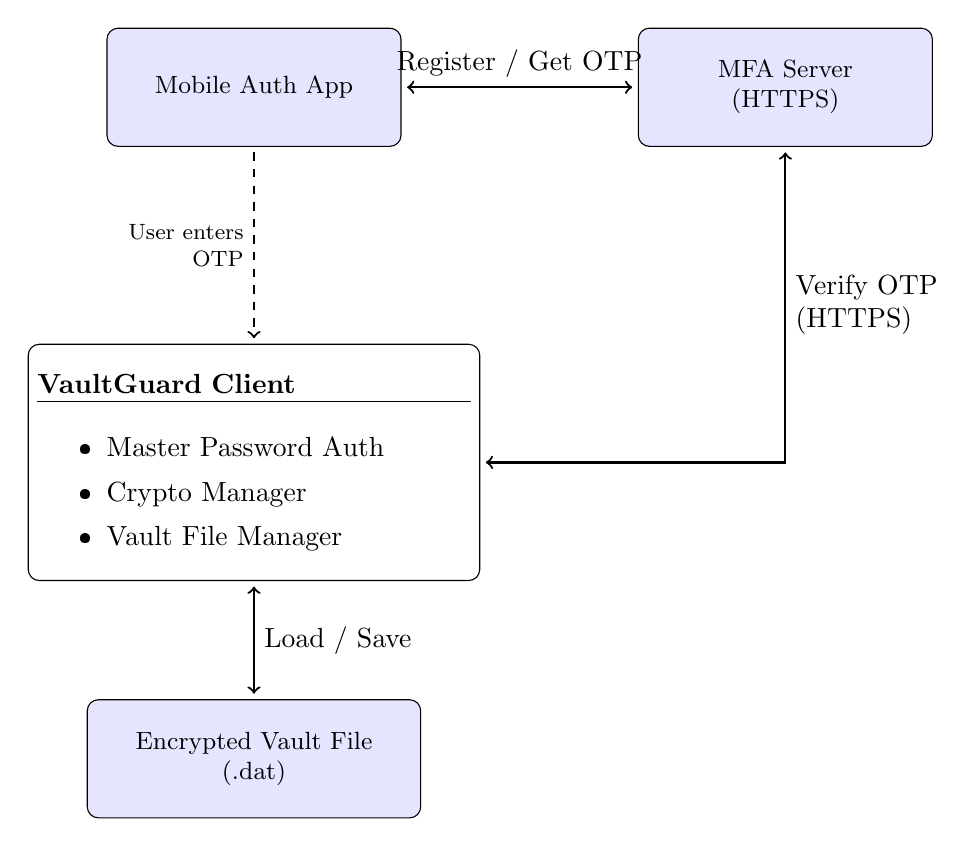
\begin{tikzpicture}[
    node distance=1.5cm and 3cm, % Increased horizontal distance
    auto,
    block/.style={
        rectangle,
        draw,
        text width=3.5cm,
        align=center,
        rounded corners,
        minimum height=1.5cm,
        fill=blue!10,
        font=\small
    },
    line/.style={
        draw,
        thick,
        -latex',
        shorten >=2pt,
        shorten <=2pt
    },
    clientbox/.style={
        rectangle,
        draw,
        text width=5.5cm,
        align=left,
        rounded corners,
        minimum height=3cm,
        fill=white
    }
]

% Nodes
\node [block] (mobile) {Mobile Auth App};
\node [block, right=of mobile] (server) {MFA Server\\(HTTPS)};

\node [clientbox, below=of mobile, yshift=-1cm] (client) {
    \textbf{VaultGuard Client}
    \vspace{0.1cm}
    \hrule
    \vspace{0.1cm}
    \begin{itemize}
        \setlength\itemsep{0em}
        \item Master Password Auth
        \item Crypto Manager
        \item Vault File Manager
    \end{itemize}
};

\node [block, below=of client, text width=4cm] (vault) {Encrypted Vault File\\(.dat)};

% Paths
% 1. Mobile <-> Server
\path [line, <->] (mobile) -- node [above, align=center] {Register / Get OTP} (server);

% 2. Client <-> Server (Horizontal then Vertical to avoid crowding)
\draw [line, <->] (client.east) -| node [near end, right, align=left] {Verify OTP\\(HTTPS)} (server.south);

% 3. Client <-> Vault
\path [line, <->] (client) -- node [right] {Load / Save} (vault);

% 4. Conceptual user flow
\draw [line, dashed, ->] (mobile.south) -- node [left, font=\footnotesize, align=right] {User enters\\OTP} (client.north);

\end{tikzpicture}
\caption{VaultGuard System Data Flow}
\end{figure}

\section{Security Architecture}

\subsection{Multi-Layer Security}

VaultGuard implements security across three layers:

\begin{enumerate}
    \item \textbf{Transport Layer}: SSL/TLS encryption for all network communication
    \item \textbf{Application Layer}: Strong authentication and authorization checks
    \item \textbf{Storage Layer}: AES-256-GCM encryption with integrity verification
\end{enumerate}

\subsection{Authentication Flow}

\begin{figure}[!ht]
\centering
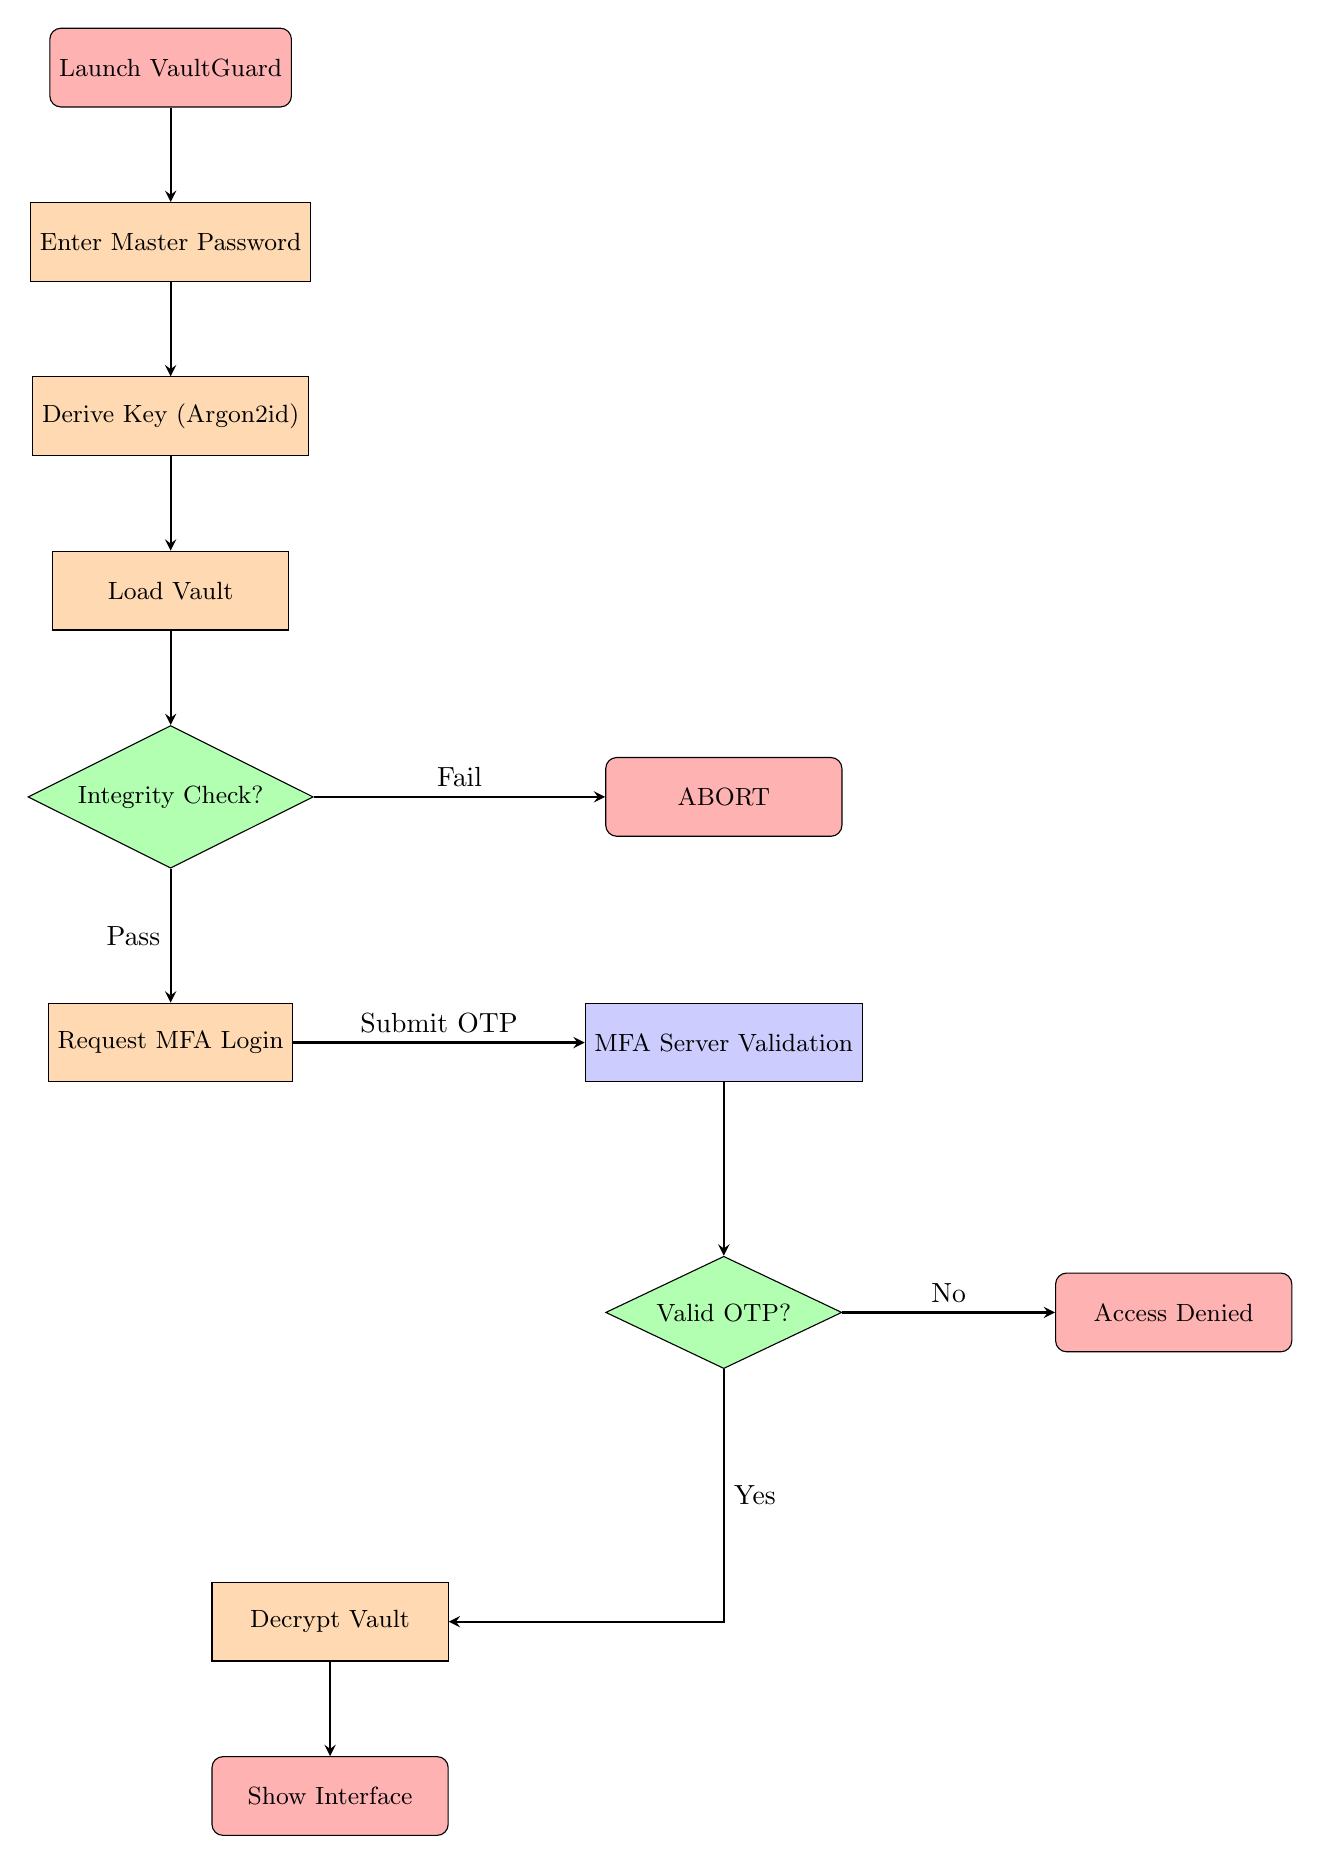
\begin{tikzpicture}[
    node distance=1.2cm,
    auto,
    startstop/.style={rectangle, rounded corners, minimum width=3cm, minimum height=1cm, text centered, draw=black, fill=red!30, font=\small},
    process/.style={rectangle, minimum width=3cm, minimum height=1cm, text centered, draw=black, fill=orange!30, font=\small},
    decision/.style={diamond, aspect=2, minimum width=3cm, minimum height=1cm, text centered, draw=black, fill=green!30, font=\small},
    arrow/.style={thick,->,>=stealth}
]

\node (start) [startstop] {Launch VaultGuard};
\node (in1) [process, below=of start] {Enter Master Password};
\node (pro1) [process, below=of in1] {Derive Key (Argon2id)};
\node (pro2) [process, below=of pro1] {Load Vault};
\node (dec1) [decision, below=of pro2] {Integrity Check?};
\node (stop1) [startstop, right=of dec1, xshift=2.5cm] {ABORT};

\node (pro3) [process, below=of dec1, yshift=-0.5cm] {Request MFA Login};
\node (server) [process, right=of pro3, xshift=2.5cm, fill=blue!20] {MFA Server Validation};

\node (dec2) [decision, below=of server, yshift=-1cm] {Valid OTP?};
\node (stop2) [startstop, right=of dec2, xshift=1.5cm] {Access Denied};
\node (pro4) [process, below=of dec2, yshift=-1.5cm, xshift=-5cm] {Decrypt Vault};
\node (end) [startstop, below=of pro4] {Show Interface};

% Arrows
\draw [arrow] (start) -- (in1);
\draw [arrow] (in1) -- (pro1);
\draw [arrow] (pro1) -- (pro2);
\draw [arrow] (pro2) -- (dec1);
\draw [arrow] (dec1) -- node[anchor=south] {Fail} (stop1);
\draw [arrow] (dec1) -- node[anchor=east] {Pass} (pro3);
\draw [arrow] (pro3) -- node[anchor=south] {Submit OTP} (server);
\draw [arrow] (server) -- (dec2);
\draw [arrow] (dec2) -- node[anchor=south] {No} (stop2);

% Routing for "Yes" branch
\draw [arrow] (dec2.south) |- node[anchor=west, near start] {Yes} (pro4.east);
\draw [arrow] (pro4) -- (end);

\end{tikzpicture}
\caption{VaultGuard Authentication Flow}
\end{figure}

\chapter{Technical Implementation}

\section{Project Directory Structure}

The project follows a modular architecture to separate concerns and improve maintainability.

\dirtree{%
.1 security/.
.2 src/.
.3 auth/.
.4 mfa\_server.py\DTcomment{MFA HTTPS server}.
.4 mfa\_client.py\DTcomment{MFA client library}.
.3 cli/.
.4 main.py\DTcomment{CLI entry point}.
.4 mobile\_auth\_app.py\DTcomment{Mobile CLI simulator}.
.3 core/.
.4 crypto\_manager.py\DTcomment{Core cryptography}.
.4 vault\_file\_manager.py\DTcomment{File I/O and integrity}.
.3 gui/.
.4 vault\_gui.py\DTcomment{Main desktop GUI}.
.4 mobile\_auth\_gui.py\DTcomment{Mobile app GUI}.
.3 utils/.
.2 data/.
.3 vault.dat\DTcomment{Encrypted vault storage}.
.3 mfa\_db.json\DTcomment{MFA user database}.
.2 docs/\DTcomment{Project documentation}.
.2 scripts/\DTcomment{Batch helper scripts}.
.2 tests/\DTcomment{Unit and integration tests}.
.2 README.md\DTcomment{Documentation}.
}

\section{Cryptographic Algorithms}

\subsection{Key Derivation Function (KDF): Argon2id}

Argon2id is used to derive a 256-bit encryption key from the user's master password:

\begin{table}[H]
\centering
\begin{tabular}{|l|c|}
\hline
\textbf{Parameter} & \textbf{Value} \\
\hline
Algorithm & Argon2id (hybrid version) \\
Memory Cost & 65,536 KiB (64 MB) \\
Time Cost & 3 iterations \\
Parallelism & 4 threads \\
Hash Length & 32 bytes (256 bits) \\
Salt Length & 16 bytes \\
\hline
\end{tabular}
\caption{Argon2id Configuration Parameters}
\end{table}

The Argon2id parameters ensure strong resistance against both GPU and ASIC attacks:

\[
\text{Key} = \text{Argon2id}(\text{Password}, \text{Salt}, M, T, P, L)
\]

\subsection{Symmetric Encryption: AES-256-GCM}

All credentials are encrypted using AES-256 in Galois/Counter Mode:

\begin{table}[H]
\centering
\begin{tabular}{|l|c|}
\hline
\textbf{Parameter} & \textbf{Value} \\
\hline
Algorithm & AES (Advanced Encryption Standard) \\
Key Size & 256 bits \\
Mode & GCM (Galois/Counter Mode) \\
Nonce Size & 96 bits (12 bytes) \\
Authentication Tag & Built-in AEAD \\
\hline
\end{tabular}
\caption{AES-256-GCM Configuration}
\end{table}

\subsection{Hash Function: SHA-256}

SHA-256 is used for vault file integrity verification:

\[
\text{FileHash} = \text{SHA-256}(\text{EncryptedVaultData})
\]

\subsection{TOTP Implementation}

Time-based One-Time Password (RFC 6238) with 60-second interval:

\[
\text{OTP} = \text{HMAC-SHA1}(\text{Secret}, \lfloor T/60 \rfloor) \bmod 10^6
\]

\section{Implementation Details}

\subsection{Vault Encryption Process}

\begin{lstlisting}[language=Python, caption=Vault Encryption Implementation]
def encrypt_vault_data(self, plaintext: str, encryption_key: bytes) -> dict:
    # Generate random 96-bit nonce
    nonce = os.urandom(12)
    
    # Create AES-GCM cipher
    aesgcm = AESGCM(encryption_key)
    
    # Encrypt data (GCM provides authentication)
    ciphertext = aesgcm.encrypt(nonce, plaintext.encode('utf-8'), None)
    
    return {
        'ciphertext': b64encode(ciphertext).decode('utf-8'),
        'nonce': b64encode(nonce).decode('utf-8')
    }
\end{lstlisting}

\subsection{Master Password Hashing}

\begin{lstlisting}[language=Python, caption=Argon2id Password Hashing]
def hash_master_password(self, password: str) -> str:
    # Hash using Argon2id with secure parameters
    return self.ph.hash(password)
    # Parameters configured in __init__:
    # time_cost=3, memory_cost=65536, parallelism=4
\end{lstlisting}

\subsection{TOTP-based MFA}

\begin{lstlisting}[language=Python, caption=TOTP Verification on MFA Server]
@app.route('/login', methods=['POST'])
def login():
    username = request.json.get('username')
    otp_code = request.json.get('otp')
    
    user = users_db.get(username)
    secret = user['secret']
    
    # Verify OTP with 60-second interval
    totp = pyotp.TOTP(secret, interval=60)
    
    # Allow +/- one interval for clock drift
    if totp.verify(otp_code, valid_window=1):
        return jsonify({"authenticated": True})
    else:
        return jsonify({"authenticated": False}), 401
\end{lstlisting}

\section{Dual Transfer OTP Mechanism}

The MFA system implements a dual-transfer mechanism where:

\begin{enumerate}
    \item Server generates OTP using TOTP and stored secret
    \item Mobile Authenticator App fetches current OTP from server
    \item VaultGuard Client also fetches OTP from server
    \item Both receive the same OTP code within the 60-second window
    \item User enters OTP in VaultGuard for authentication
\end{enumerate}

This ensures that OTP generation is server-controlled while both applications have access to the same code.

\chapter{Security Analysis}

\section{Threat Model}

\subsection{Threats Addressed}

\begin{table}[H]
\centering
\begin{tabular}{|p{3cm}|p{4cm}|p{4cm}|}
\hline
\textbf{Threat} & \textbf{Attack Vector} & \textbf{Mitigation} \\
\hline
Brute Force & Dictionary/exhaustive password search & Argon2id with high memory cost \\
Network Eavesdropping & Man-in-the-middle on HTTP & SSL/TLS encryption \\
Data Tampering & Modifying vault file & SHA-256 integrity verification \\
Offline Attack & Compromised vault file & AES-256-GCM + strong KDF \\
Replay Attack & Reusing old OTP codes & 60-second validity window \\
Weak Passwords & User choosing simple passwords & No mitigation (user responsibility) \\
\hline
\end{tabular}
\caption{Threat Model and Mitigations}
\end{table}

\section{Security Strength Analysis}

\subsection{Master Password Security}

Using Argon2id with the configured parameters:

\begin{enumerate}
    \item \textbf{Memory Hardness}: 64 MB memory requirement makes GPU/ASIC attacks expensive
    \item \textbf{Time Hardness}: 3 iterations add computational overhead
    \item \textbf{Salting}: 16-byte random salt prevents rainbow table attacks
    \item \textbf{Hybrid Mode}: Argon2id combines benefits of data-independent and dependent variants
\end{enumerate}

\subsection{Encryption Security}

AES-256-GCM provides:

\begin{enumerate}
    \item \textbf{256-bit key}: $2^{256}$ possible keys (computationally infeasible to brute force)
    \item \textbf{GCM mode}: Authenticated encryption prevents tampering
    \item \textbf{Random nonce}: Ensures different ciphertexts for same plaintext
\end{enumerate}

\chapter{Testing and Validation}

\section{Test Strategy}

VaultGuard implements a comprehensive testing strategy covering:

\begin{enumerate}
    \item \textbf{Unit Tests}: Individual component testing
    \item \textbf{Integration Tests}: End-to-end workflow testing
    \item \textbf{Security Tests}: Cryptographic algorithm validation
    \item \textbf{Tampering Tests}: Data integrity verification
\end{enumerate}

\section{Test Results Summary}

\subsection{Overall Test Statistics}

\begin{table}[H]
\centering
\begin{tabular}{|l|c|c|c|}
\hline
\textbf{Test Suite} & \textbf{Tests Run} & \textbf{Passed} & \textbf{Failed} \\
\hline
Cryptography Module & 3 & 3 & 0 \\
Argon2 KDF & 8 & 8 & 0 \\
MFA/TOTP System & 6 & 6 & 0 \\
Vault File Manager & 4 & 4 & 0 \\
Integration Tests & 3 & 3 & 0 \\
\hline
\textbf{TOTAL} & \textbf{24} & \textbf{24} & \textbf{0} \\
\hline
\end{tabular}
\caption{Test Results Summary}
\end{table}

\textbf{Test Success Rate: 100\%}

\section{Detailed Test Cases}

\subsection{Cryptography Module Tests}

\begin{lstlisting}[caption=Test Case: Encrypt/Decrypt Cycle]
def test_encrypt_decrypt(self):
    plaintext = [
        {"service": "Gmail", "username": "user", "password": "pass"}
    ]
    encrypted = crypto.encrypt_data(plaintext, "master_password")
    decrypted = crypto.decrypt_data(encrypted, "master_password")
    assert decrypted == plaintext  # PASS
\end{lstlisting}

\chapter{Conclusion}

VaultGuard successfully demonstrates the implementation of a secure password management system incorporating industry-standard cryptographic practices. The project integrates multiple security technologies including Argon2id key derivation, AES-256-GCM encryption, TOTP-based MFA, SSL/TLS secured communication, and SHA-256 integrity verification. All components have been thoroughly tested with 24 comprehensive test cases, achieving 100\% pass rate.

\chapter*{References}

\begin{thebibliography}{99}
\bibitem{nist2016} NIST, ``Recommendation for Password-Based Key Derivation,'' NIST Special Publication 800-132, 2016.
\bibitem{gcm2007} McGrew, D., ``The Security and Performance of the Galois/Counter Mode (GCM),'' 2007.
\bibitem{rfc6238} IETF, ``Time-Based One-Time Password Algorithm,'' RFC 6238, 2011.
\bibitem{argon2} Biryukov, A., ``Argon2: the memory-hard password hash,'' 2015.
\end{thebibliography}

\appendix

\chapter{Installation and Setup Guide}

\section{System Requirements}
\begin{itemize}
    \item Python 3.8 or higher, Windows OS, 2GB RAM.
\end{itemize}

\section{Installation Steps}
\begin{lstlisting}[language=bash]
# Install dependencies
install_deps.bat

# Run the GUI system (MFA Server + Mobile App + Vault Client)
start_gui.bat
\end{lstlisting}

\chapter{User Manual}

\section{Using VaultGuard}
\begin{enumerate}
    \item Run \texttt{start\_gui.bat}.
    \item In the Mobile Authenticator window, click "Register New Device", enter a username.
    \item In the VaultGuard Client window, enter your Master Password (new or existing).
    \item Enter the same username and the 6-digit OTP displayed in the Mobile App.
    \item Access your secure vault.
\end{enumerate}

\end{document}
